\chapter{Facet Joint Injection}

\section*{Overview}
Facet joints are small joints along the back of the spine that help guide movement. A facet joint injection places medicine into one of these joints. A related but different procedure, a medial branch block, injects local anesthetic near the small nerves that carry signals from the joints. These procedures may be used to assess or treat selected neck or back pain, but a response does not prove that a facet joint is the only cause of pain.


\begin{center}
\begin{minipage}{\textwidth}\centering
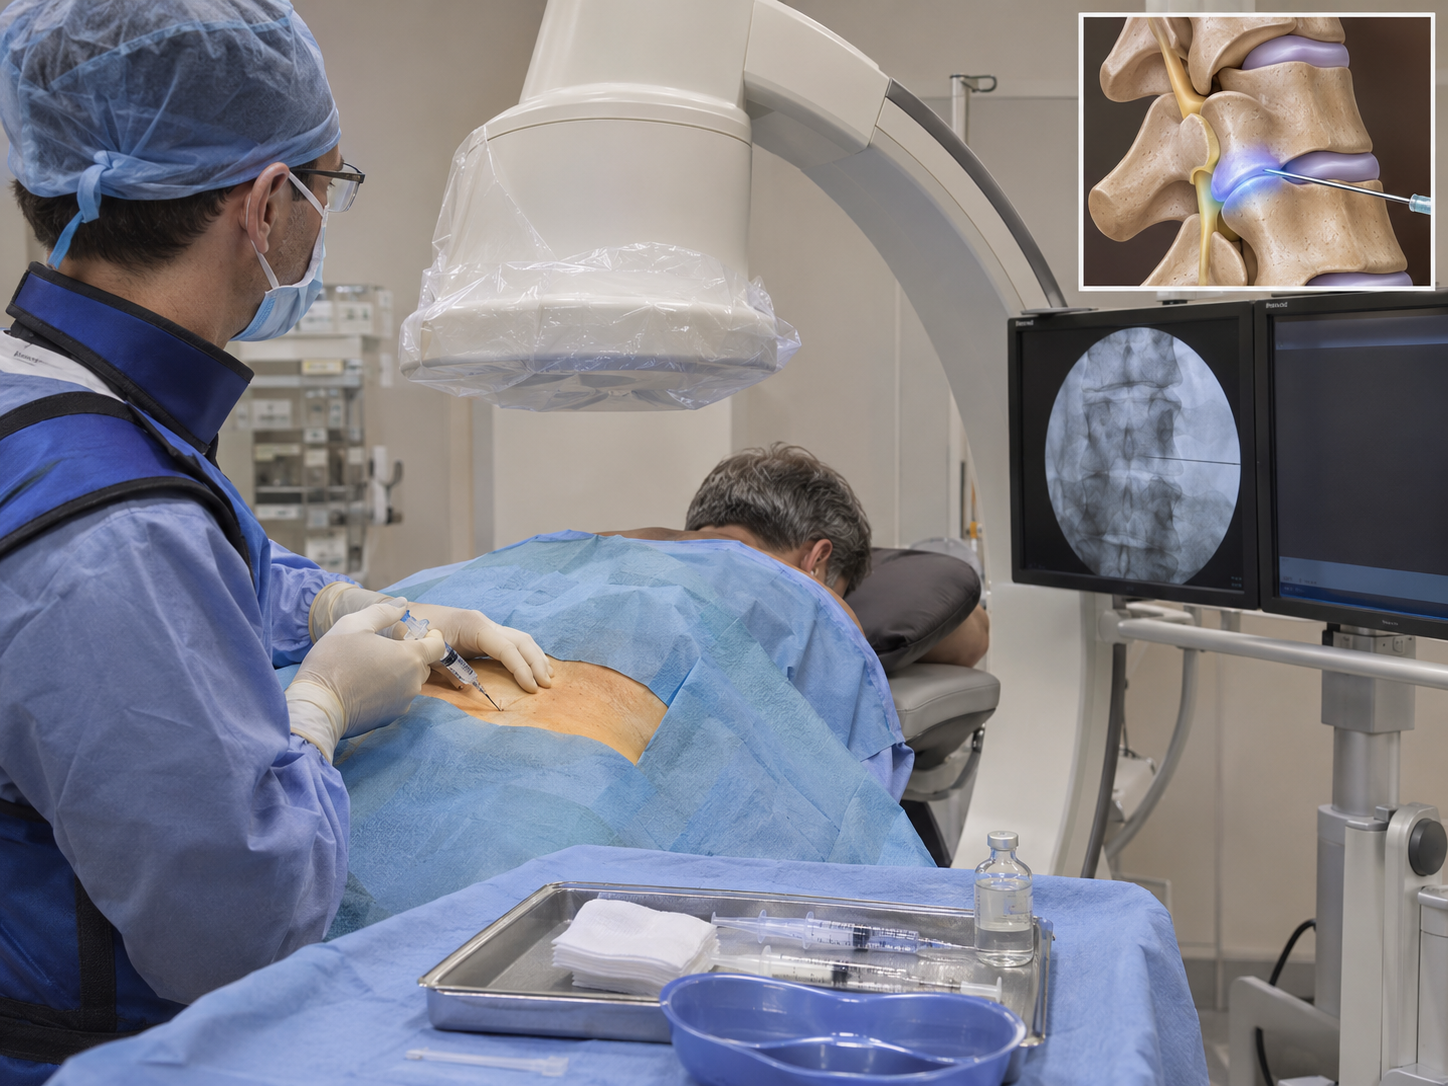
\includegraphics[width=0.82\textwidth]{images/chapters/procedure_facet_joint_injection_overview.png}
\captionof{figure}{Facet Joint Injection: A clinician performs a spine injection with imaging guidance.}
\end{minipage}
\end{center}
\section*{Common Instruments and Equipment}
The exact setup varies by technique and setting. Common items may include:
\begin{itemize}[nosep,leftmargin=*]
  \item spinal needle and syringe
  \item fluoroscopy or CT guidance when used
  \item contrast and sterile preparation supplies
\end{itemize}

\section*{Alternative Names}
Facet joint injection; intra-articular facet injection; zygapophyseal joint injection; facet block. Medial branch block (MBB) is a related procedure that targets the nerve supplying the joint rather than the joint itself.

\section*{Principle}
An intra-articular injection places local anesthetic, sometimes with corticosteroid, inside the facet joint. An MBB places a small amount of local anesthetic near the medial branch nerve. Pain relief after an MBB is used as a temporary screening result to help decide whether radiofrequency ablation of the nerve may be appropriate. Relief is not a definitive diagnosis because medicine can spread to nearby tissues, symptoms vary, and other factors can affect pain.

\section*{History}
Facet injections and medial branch blocks have been used for decades in the assessment and management of spinal pain. Their best role remains debated. Current practice guidelines distinguish joint injections from nerve blocks and generally favor medial branch blocks when selecting people for radiofrequency treatment.

\section*{Why It Is Done}
An injection may be considered for persistent pain thought to come from facet joints in the neck, mid-back, or lower back, usually after other treatments have not helped enough. Guidance differs: NICE advises against spinal injections to manage low back pain. A 2026 multisociety guideline notes that a steroid injection may provide short- to intermediate-term relief for a small subset of people, such as those with an acute injury or evidence of active facet-joint inflammation. An MBB is commonly used to see whether short-term numbing of the joint's nerve supply reduces pain and improves movement; in the UK, NICE supports considering radiofrequency denervation for selected people with chronic low back pain after a positive diagnostic MBB. These injections are not intended to treat pain caused by pressure on a spinal nerve, such as typical sciatica.

\section*{Role in Care}
These are image-guided diagnostic or treatment procedures, not first-line care. Pain history, physical examination, and scans cannot reliably identify a painful facet joint by themselves. A clinician may recommend exercise-based rehabilitation and other noninvasive treatments before considering an injection. Which procedure is chosen depends on the pain pattern, prior care, and the treatment question.

\section*{How It Is Performed}
The procedure is usually done in an outpatient clinic with X-ray (fluoroscopy) or CT guidance. The person lies face down or in another position that gives access to the target. After cleaning the skin and numbing it, the clinician guides a needle either into the joint or near its medial branch nerve. A small amount of contrast dye may be used to check placement. The clinician then injects the planned medicine and removes the needle. The number of levels treated and the medicines used depend on the purpose of the procedure. Sedation is not routinely needed for a diagnostic MBB because it can affect the assessment; any exception is discussed in advance.

\section*{Preparation}
The clinic reviews the reason for the injection, medicines, allergies, prior imaging, and health conditions. Tell the team about blood thinners, diabetes, infection, pregnancy or possible pregnancy, and allergies to contrast, local anesthetic, or steroid. Blood-thinning medicines do not need to be stopped automatically; the clinician and prescribing team decide whether any change is needed for the specific procedure. Follow instructions about eating, drinking, and transportation, especially if sedation is planned.

\section*{Contraindications}
An active infection or an unsafe bleeding risk may mean the procedure should be postponed or modified.

\section*{Precautions}
Diabetes is relevant because corticosteroids may temporarily raise blood sugar. A diagnostic block should be done in a way that does not unnecessarily obscure the pain response. Allergy to a planned medicine or contrast may require another approach. Neck-joint injections need particular care because nearby blood vessels and nerves make an accidental injection into a blood vessel more dangerous; clinicians use imaging and choose medicines with this risk in mind. The clinician also considers prior spine surgery, anatomy, pregnancy, and whether the result will answer a useful treatment question.

\section*{Risks}
Temporary soreness, bruising, or a brief increase in pain can occur. Local anesthetic may temporarily cause numbness or weakness. Corticosteroid may cause a temporary increase in blood sugar, flushing, or other steroid effects. Uncommon complications include bleeding, infection, allergic reaction, nerve irritation, or injury to nearby structures. Serious spinal injury is rare but possible. Repeated steroid exposure has risks, so injections are not given as an automatic series.

\section*{Aftercare and Recovery}
The clinic may observe the person briefly and provide instructions about activity and driving. If local anesthetic was used, numbness or pain relief may occur briefly and then wear off. For a diagnostic MBB, record pain and function during the period specified by the clinic, often using a diary; the numbing medicine is expected to provide temporary relief. Steroid effects, if any, may take several days and are not guaranteed. People with diabetes may need to monitor blood sugar as directed.

\section*{Outcome and Results}
The clinician reviews how much pain changed, how long relief lasted, and whether usual activities became easier. A temporary response to an MBB can support consideration of radiofrequency ablation, but it does not establish a certain diagnosis or guarantee that ablation will help. The amount of relief and number of diagnostic blocks needed before ablation vary among guidelines, clinicians, and health systems. Intra-articular steroid injections may help some selected patients, but lasting benefit is not assured and routine repeated treatment is not recommended for everyone.

\section*{Expected Results}
The goal may be temporary pain relief or information to guide another treatment. Some people have meaningful short-term improvement; others have little or none. An injection does not repair arthritis or reverse other changes in the spine, and it may not reduce pain arising from multiple sources.

\section*{Follow-up}
Follow up with the ordering clinician to review the response and next steps. Options may include continued rehabilitation, medication or activity changes, another diagnostic block, radiofrequency ablation for selected people, or further evaluation. Repeat steroid injection is considered individually rather than scheduled as a routine series.

\section*{When to Seek Medical Care}
Contact the clinic for increasing redness, warmth, swelling, or drainage at the injection site, fever, or persistent severe pain. Seek urgent care for new or worsening leg or arm weakness, loss of coordination, numbness around the groin, loss of bladder or bowel control, severe headache, trouble breathing, or rapidly worsening symptoms.

\section*{References}
\begin{enumerate}
  \item Cohen SP, Bhaskar A, Bhatia A, et al. Consensus practice guidelines on interventions for lumbar facet joint pain from a multispecialty, international working group. Regional Anesthesia and Pain Medicine. 2020;45:424--467. https://pmc.ncbi.nlm.nih.gov/articles/PMC7362874/
  \item Provenzano DA, et al. Multisociety multispecialty consensus recommendations on corticosteroid injections for facet joint and sacroiliac joint pain. Regional Anesthesia and Pain Medicine. 2026. https://rapm.bmj.com/content/early/2026/01/22/rapm-2025-107347
  \item Guy's and St Thomas' NHS Foundation Trust. Facet joint injections for treating pain. https://www.guysandstthomas.nhs.uk/health-information/facet-joint-injections-treating-pain
  \item National Institute for Health and Care Excellence. Low back pain and sciatica in over 16s: assessment and management. https://www.nice.org.uk/guidance/ng59/chapter/recommendations
\end{enumerate}

\clearpage
